\documentclass[11pt,a4paper]{article}
\usepackage[T1]{fontenc}
\usepackage[utf8]{inputenc}
\usepackage[english]{babel}
\usepackage[a4paper,top=2cm,bottom=2cm,left=2.1cm,right=2.1cm]{geometry}
\usepackage{amsmath,amssymb,mathtools}
\usepackage{graphicx}
\usepackage{booktabs,array,tabularx}
\usepackage{xcolor}
\usepackage{microtype}
\usepackage{enumitem}
\usepackage{tcolorbox}
\usepackage{tikz}
\usetikzlibrary{arrows.meta,positioning,calc,shapes.geometric}
\usepackage{caption}
\usepackage{pdflscape}
\usepackage[colorlinks=true,allcolors=blue!55!black]{hyperref}
\microtypesetup{expansion=false}
\setlength{\parindent}{0pt}
\setlength{\parskip}{5pt}
\definecolor{infected}{HTML}{C43B3B}
\definecolor{exact}{HTML}{2878B5}
\definecolor{macro}{HTML}{E07A1F}
\definecolor{boundary}{HTML}{429C74}
\definecolor{purple}{HTML}{7F5AA2}
\definecolor{soft}{HTML}{F6F8FA}
\tikzset{
 inode/.style={circle,draw=infected,fill=infected,minimum size=7mm,inner sep=0pt},
 snode/.style={circle,draw=gray!65,fill=gray!18,minimum size=7mm,inner sep=0pt},
 ibnode/.style={circle,draw=exact,line width=1.3pt,fill=infected,minimum size=7mm,inner sep=0pt},
 sbnode/.style={circle,draw=exact,line width=1.3pt,fill=gray!18,minimum size=7mm,inner sep=0pt}
}
\title{\textbf{How Full Micro, MicroMacro, and Structural A/U--E/U--E/E Actually Work}\\[4pt]
\large A step-by-step explanation using one network, formulas, implementation details, and comparison results}
\author{}
\date{}
\begin{document}
\maketitle

\begin{tcolorbox}[colback=soft,colframe=boundary,title=What this document is meant to clarify]
All variants below simulate infection spreading on a network, but they use different amounts of information about inter-community contacts. \textbf{Full Micro} sees every edge. \textbf{Production MicroMacro} keeps detailed node-level networks inside communities but uses aggregate information between communities. \textbf{Structural A/U, E/U, and E/E} are diagnostic variants in which the information lost by aggregation is restored one component at a time.
\end{tcolorbox}

\section*{1. Start from the same physical network}
Assume two communities, A and B. Each contains an ordinary person-to-person contact network. Only a few real contacts connect the two communities. Red nodes are infected, gray nodes are susceptible. A blue outline marks a boundary/gateway node that has at least one contact with another community.

\begin{figure}[h!]
\centering
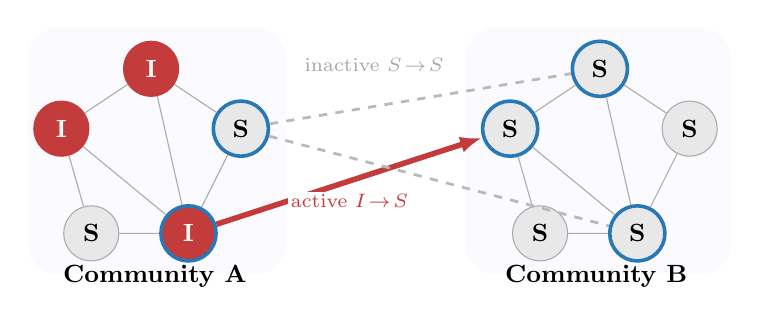
\begin{tikzpicture}[scale=.95,every node/.style={font=\small}]
\fill[blue!2,rounded corners=4mm] (-0.45,-0.55) rectangle (3.0,2.75);
\fill[blue!2,rounded corners=4mm] (5.4,-0.55) rectangle (8.95,2.75);
\node[inode,text=white,font=\bfseries\small] (a1) at (0,1.4) {I};
\node[inode,text=white,font=\bfseries\small] (a2) at (1.2,2.2) {I};
\node[sbnode,font=\bfseries\small] (a3) at (2.4,1.4) {S};
\node[snode,font=\bfseries\small] (a4) at (0.4,0.0) {S};
\node[ibnode,text=white,font=\bfseries\small] (a5) at (1.7,0.0) {I};
\draw[gray!65] (a1)--(a2)--(a3)--(a5)--(a4)--(a1); \draw[gray!65] (a1)--(a5); \draw[gray!65] (a2)--(a5);
\node[font=\bfseries\small] at (1.25,-0.58) {Community A};
\node[sbnode,font=\bfseries\small] (b1) at (6.0,1.4) {S};
\node[sbnode,font=\bfseries\small] (b2) at (7.2,2.2) {S};
\node[snode,font=\bfseries\small] (b3) at (8.4,1.4) {S};
\node[snode,font=\bfseries\small] (b4) at (6.4,0.0) {S};
\node[sbnode,font=\bfseries\small] (b5) at (7.7,0.0) {S};
\draw[gray!65] (b1)--(b2)--(b3)--(b5)--(b4)--(b1); \draw[gray!65] (b1)--(b5); \draw[gray!65] (b2)--(b5);
\node[font=\bfseries\small] at (7.15,-0.58) {Community B};
\draw[line width=2pt,infected,-{Latex[length=2.8mm]}] (a5)--node[below=1mm,fill=white,inner sep=1pt,font=\scriptsize,text=infected] {active $I\!\to\!S$} (b1);
\draw[line width=1pt,gray!55,dashed] (a3)--(b2); \draw[line width=1pt,gray!55,dashed] (a3)--(b5);
\node[font=\scriptsize,text=gray!70] at (4.18,2.25) {inactive $S\!\to\!S$};
\end{tikzpicture}
\caption{One physical network. There are three cross-community edges, but only one is currently active as an $I\to S$ transmission channel. Different simulators either retain or lose this distinction.}
\end{figure}

The same physical network is supplied to all simulators. The difference is not the graph itself, but which part of the graph is used when inter-community transmission is computed.

\section*{2. Full Micro: the simulator sees everything}
Full Micro is a Gillespie simulation on the entire contact graph. It makes no physical distinction between an internal edge and a cross-community edge. Every active $I\to S$ edge is a CTMC transition channel:
\[
a_{uv}=\beta w_{uv}\,\mathbf{1}[X_u=I,\,X_v=S].
\]
The total infection hazard is the sum over all currently active channels,
\[
\Theta_{\mathrm{micro}}=\sum_{(u,v)\in E} a_{uv}.
\]
Thus Full Micro effectively asks: \emph{which particular infected people are currently connected to which particular susceptible people?}

In Fig.~1 only one of the three cross-community edges is active. If all cross-edges have weight 1 and infection rate $\beta$, the exact A$\to$B cross-community hazard is simply
\[
\lambda^{\mathrm{exact}}_{AB}=\beta.
\]
If that channel fires, the susceptible node at the actual endpoint of that edge is infected. Full Micro does not invent a target; the graph determines it.

\begin{tcolorbox}[colback=soft,colframe=exact,title=Intuition]
Full Micro = ``I know the state of every person and every edge, so I know exactly which transitions are currently possible.''
\end{tcolorbox}

\section*{3. Production MicroMacro: detailed inside communities, coarse between them}
MicroMacro keeps a node-level Gillespie process inside each community, but compresses inter-community information. At the macro layer a community is represented approximately by quantities such as
\[
A:\quad I_A,\;S_A,\;N_A,
\]
and each pair of communities has an aggregate weight $W_{AB}$.

The MoMLeT model writes the inter-community rate as
\[
\lambda_{AB}(t)=\beta W_{AB} C_A(t)S_B(t)T,
\]
where $C_A$ is aggregate contagiousness, $S_B$ is aggregate susceptibility, and $T$ is a calibration factor. A useful schematic reading is
\[
\lambda^{A/U}_{AB}\propto \beta W_{AB}\frac{I_A}{N_A}\frac{S_B}{N_B}.
\]
For the toy network, $W_{AB}=3$, $I_A/N_A=2/5$, and $S_B/N_B=1$, so an aggregate formula can give approximately
\[
\lambda^{A/U}_{AB}=3\beta\frac{2}{5}=1.2\beta,
\]
although Full Micro sees only one active cross-edge and gives $\beta$.

\begin{figure}[h!]
\centering
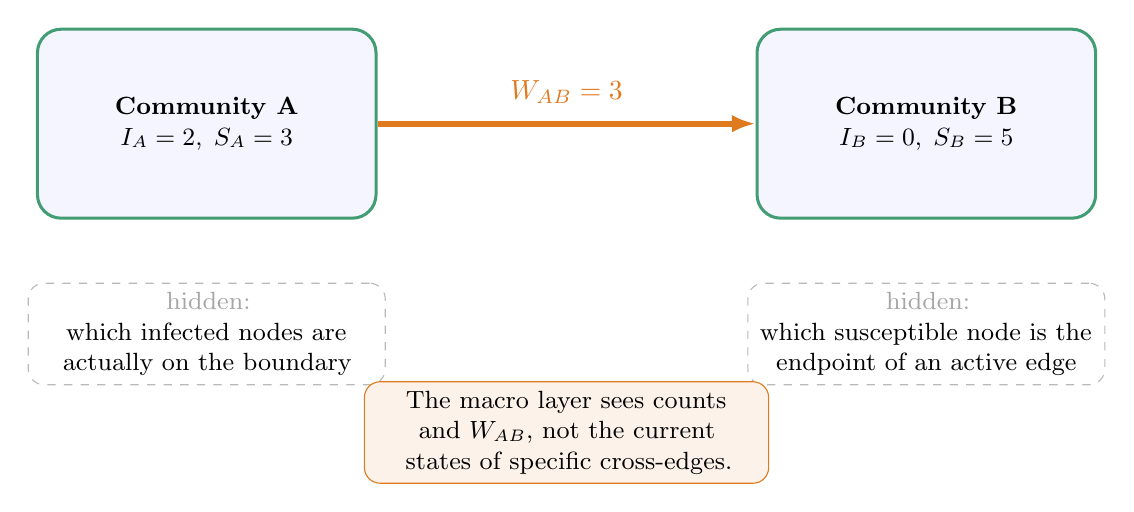
\begin{tikzpicture}[node distance=12mm,every node/.style={font=\small}]
\node[rounded corners=3mm,draw=boundary,line width=1.1pt,fill=blue!4,minimum width=43mm,minimum height=24mm,align=center] (A) {\textbf{Community A}\\$I_A=2,\;S_A=3$};
\node[rounded corners=3mm,draw=boundary,line width=1.1pt,fill=blue!4,minimum width=43mm,minimum height=24mm,align=center,right=48mm of A] (B) {\textbf{Community B}\\$I_B=0,\;S_B=5$};
\draw[-{Latex[length=3mm]},line width=2.2pt,macro] (A)--node[above=1mm,font=\bfseries] {$W_{AB}=3$} (B);
\node[draw=gray!55,dashed,rounded corners=2mm,fill=white,align=center,text width=43mm,below=8mm of A] (ha) {\textcolor{gray!70}{hidden:}\\which infected nodes are actually on the boundary};
\node[draw=gray!55,dashed,rounded corners=2mm,fill=white,align=center,text width=43mm,below=8mm of B] (hb) {\textcolor{gray!70}{hidden:}\\which susceptible node is the endpoint of an active edge};
\node[rounded corners=2mm,fill=macro!10,draw=macro,align=center,text width=49mm,below=6mm of $(ha)!0.5!(hb)$] {The macro layer sees counts and $W_{AB}$, not the current states of specific cross-edges.};
\end{tikzpicture}
\caption{Macro-level view of the same network. Node-level models still exist inside communities, but production MicroMacro uses aggregate counts and $W_{AB}$ for cross-community transmission.}
\end{figure}

This is the structural approximation: the macro layer assumes infected and susceptible nodes are mixed with respect to the boundary roughly as they are in the whole community. After a macro event, production MicroMacro does not know the exact endpoint of the physical cross-edge, so it imports infection into a uniformly selected susceptible node of the destination community.

\subsection*{3.1. A second difference: how MicroMacro advances time}
Production MicroMacro also has its own scheduler. Micro communities advance in intervals of length $\tau_{\mathrm{micro}}$, while the macro layer accumulates
\[
H(t)=\int_{t_0}^{t}\Theta(s)\,ds
\]
until it reaches a random threshold $E=-\ln U$. In the production implementation this integral is evaluated on the synchronization grid, using a midpoint-style approximation within intervals.

\begin{figure}[h!]
\centering
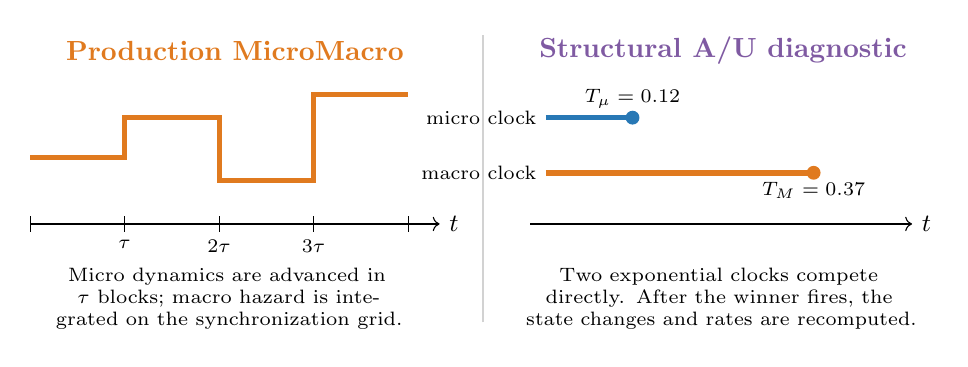
\begin{tikzpicture}[every node/.style={font=\small}]
\node[font=\bfseries,text=macro] at (2.6,3.0) {Production MicroMacro};
\draw[->] (0,0.8)--(5.2,0.8) node[right] {$t$};
\foreach \x in {0,1.2,2.4,3.6,4.8} {\draw (\x,0.9)--(\x,0.7);}
\node[below,font=\scriptsize] at (1.2,0.72) {$\tau$}; \node[below,font=\scriptsize] at (2.4,0.72) {$2\tau$}; \node[below,font=\scriptsize] at (3.6,0.72) {$3\tau$};
\draw[macro,line width=1.8pt] (0,1.65)--(1.2,1.65)--(1.2,2.15)--(2.4,2.15)--(2.4,1.35)--(3.6,1.35)--(3.6,2.45)--(4.8,2.45);
\node[align=center,text width=48mm,font=\scriptsize] at (2.5,-0.15) {Micro dynamics are advanced in $\tau$ blocks; macro hazard is integrated on the synchronization grid.};
\draw[gray!35,line width=.8pt] (5.75,-0.45)--(5.75,3.2);
\node[font=\bfseries,text=purple] at (8.8,3.0) {Structural A/U diagnostic};
\draw[->] (6.35,0.8)--(11.2,0.8) node[right] {$t$};
\draw[line width=2pt,exact] (6.55,2.15)--(7.65,2.15); \fill[exact] (7.65,2.15) circle (2.5pt);
\node[left,font=\scriptsize] at (6.55,2.15) {micro clock}; \node[above,font=\scriptsize] at (7.65,2.15) {$T_\mu=0.12$};
\draw[line width=2pt,macro] (6.55,1.45)--(9.95,1.45); \fill[macro] (9.95,1.45) circle (2.5pt);
\node[left,font=\scriptsize] at (6.55,1.45) {macro clock}; \node[below,font=\scriptsize] at (9.95,1.45) {$T_M=0.37$};
\node[align=center,text width=49mm,font=\scriptsize] at (8.75,-0.15) {Two exponential clocks compete directly. After the winner fires, the state changes and rates are recomputed.};
\end{tikzpicture}
\caption{Scheduling difference. Production MicroMacro uses $\tau$-synchronization and cumulative-hazard integration; A/U uses direct event competition.}
\end{figure}

\begin{tcolorbox}[colback=soft,colframe=macro,title=The production baseline used in v4]
For the numerical comparisons in v4, the primary production reference is \textbf{the same MicroMacro implementation with independent RNG streams for the micro communities}. This is not a new scientific model: aggregate hazard, uniform import placement, $\tau=1$, and the production scheduler are unchanged. The shared-RNG variant is retained only as a buggy historical/current reference.
\end{tcolorbox}

\section*{4. Structural A/U: the same coarse structural assumptions, but a different simulator}
A/U means
\[
A=\text{Aggregate hazard},\qquad U=\text{Uniform placement}.
\]
Structurally, A/U makes the same two coarse assumptions as production MicroMacro: cross-community hazard is computed from aggregate information rather than exact active cross-edges, and a macro import is placed uniformly among susceptible nodes in the destination community.

However, A/U is \textbf{not the same executable code}. The diagnostic implementation does not use the production $\tau$-scheduler in the same form; micro and macro events compete as event-driven stochastic clocks.

\begin{tcolorbox}[colback=soft,colframe=macro,title=Why A/U is needed]
Full Micro and production MicroMacro differ for two reasons at once. First, exact boundary-edge information is replaced by aggregate hazard and uniform placement. Second, global event competition is replaced by the production $\tau$-synchronized hazard-integration algorithm. A/U keeps the first difference but removes the second. Therefore Full Micro vs A/U primarily exposes the structural A/U approximation rather than mixing it with production scheduling mechanics.
\end{tcolorbox}

\begin{center}
\begin{tabular}{lcc}
\toprule
 & \textbf{Production MicroMacro} & \textbf{Structural A/U}\\
\midrule
Macro information & aggregate & aggregate\\
Placement & uniform susceptible & uniform susceptible\\
Hazard idea & A/U approximation & A/U approximation\\
Time scheduler & production $\tau$ + hazard integral & event-driven clocks\\
Executable & user-facing production simulator & separate diagnostic simulator\\
\bottomrule
\end{tabular}
\end{center}

\subsection*{4.1. What the A/U comparison showed}
The baseline uses 100 paired networks with $L=10$, $n=100$, $d\approx6$, $k=5$, $\beta_{\mathrm{in}}=\beta_{\mathrm{out}}=0.003$, SI dynamics, and $T_{\mathrm{end}}=4000$.

\subsubsection*{What RMST means here}
RMST is the Restricted Mean Survival Time. In this experiment the event is the first arrival of infection in the final community of the chain. For replication $r$, let this time be $T_{\mathrm{last}}^{(r)}$. With a finite observation horizon,
\[
\mathrm{RMST}=\frac{1}{R}\sum_{r=1}^{R}\min\!\left(T_{\mathrm{last}}^{(r)},T_{\mathrm{end}}\right).
\]
For example, three runs with terminal arrival times 2800, 3200, and ``not reached by 4000'' contribute 2800, 3200, and 4000, giving RMST $=3333.3$. If every run finishes before the horizon, RMST is simply the ordinary mean terminal-arrival time.

\textbf{Interpretation:} larger RMST means slower propagation to the end of the chain. In the previous tables, $\Delta\mathrm{RMST}=\mathrm{RMST}_{\mathrm{variant}}-\mathrm{RMST}_{\mathrm{Full\ Micro}}$.

\begin{tcolorbox}[colback=white,colframe=boundary,title=v4 reporting rule]
The v4 comparison does not rely on separate small RMST tables. All six implementations are compared together in Section~8 using the full empirical distributions of $T_{\mathrm{last}}$. RMST is retained here only as historical context from earlier experiment reports.
\end{tcolorbox}

A/U reached the terminal community about 221 time units earlier than Full Micro on average ($\Delta\mathrm{RMST}\approx-220.8$; 95\% CI approximately $[-315.5,-126.8]$). This already shows that aggregate hazard plus uniform placement produces systematic acceleration even without the production scheduler.

The old shared-RNG production MicroMacro was much faster still: RMST 1677.55. The gap between it and event-driven A/U was about 1038 RMST units. That gap, however, must \textbf{not} be interpreted as a pure $\tau$-scheduler error. After correcting the shared-RNG architecture, production RMST became 2729.43 and differed from A/U by only about 13.5 RMST units; the corresponding confidence interval included zero. Reducing $\tau$ from 1 to 0.25 changed RMST by only about 31.15.

\subsubsection*{What ``Production + independent RNG streams'' means}
These are not two scientific models. Both variants use the same production MicroMacro: the same local MicroModels, aggregate macro hazard, uniform import placement, $\tau=1$, midpoint/cumulative-hazard scheduler, and normal repeated imports. The only change is the source of random numbers used by each micro community.

In the current/shared-RNG implementation, MicroModels are created without private RNG objects, so multiple communities use the same module-level Python RNG state. A shared pseudorandom generator alone is not necessarily wrong. The problem appears in combination with \textbf{horizon-safe rollback}. When \texttt{simulate\_until(t\_end)} samples a Gillespie event beyond the current horizon, it restores the RNG to the state before the draw. With a private RNG this is local. With a shared global RNG, rolling back one community also rewinds the random stream that a later community will see.

\begin{tcolorbox}[colback=soft,colframe=macro,title=Why this creates artificial dependence]
Suppose the global RNG state is $R$ before community A is simulated. A draws a future event, finds it beyond the horizon, and restores the RNG back to $R$. Community B is simulated next and starts from that same restored state. It can therefore reuse the same random-number sequence. B's stochastic evolution becomes dependent on whether A attempted and rolled back a draw. This is cross-community RNG coupling and execution-order dependence, not a physical interaction between communities.
\end{tcolorbox}

With independent streams, each micro community has its own generator,
\[
\mathrm{RNG}_1,\mathrm{RNG}_2,\ldots,\mathrm{RNG}_L.
\]
Rollback in community $i$ modifies only $\mathrm{RNG}_i$. Midpoint clones also copy and restore the corresponding per-community RNG state. Macro budget and macro pair selection remain part of the original production machinery; the scientific aggregate A/U semantics and the $\tau$-scheduler are unchanged.

A dedicated unit diagnostic confirmed the effect: two identical isolated micro processes had correlation of final infected counts about 0.531 with the shared-global RNG and about $-0.002$ with independent streams. More importantly, the probability of infecting the target was about 0.394 for the first community but only 0.155 for the second under shared RNG; after splitting the streams the values were about 0.394 and 0.390. Thus shared RNG plus rollback changed even the marginal distribution of the second community.

\begin{center}
\small
\begin{tabularx}{\textwidth}{>{\raggedright\arraybackslash}p{31mm} X X X}
\toprule
\textbf{Implementation} & \textbf{Micro scheduling/state} & \textbf{Cross-community model} & \textbf{RNG architecture}\\
\midrule
Full Micro & one global Gillespie process on the full graph & exact active edges, exact endpoint & one RNG for one global process\\
Current Production MM & separate MicroModels + $\tau$ synchronization & aggregate hazard + uniform import & one shared global RNG across micro communities\\
Production + independent RNG & same production scheduler & same aggregate/uniform model & separate RNG for each micro community\\
Structural A/U & one diagnostic global state; event-driven race & aggregate hazard + uniform placement & diagnostic streams by stochastic role\\
E/U, E/E & same diagnostic event-driven framework & exact hazard; E/U uniform, E/E exact placement & diagnostic streams; not production per-community architecture\\
\bottomrule
\end{tabularx}
\end{center}

\section*{5. E/U: correct only the hazard}
E/U keeps uniform placement but restores exact information about real cross-community edges. For pair A$\to$B,
\[
\lambda^{E/U}_{AB}=\beta\sum_{(u,v)\in E_{AB}}w_{uv}\mathbf{1}[X_u=I,\,X_v=S].
\]
In the toy network only one cross-edge is active, so $\lambda^{E/U}_{AB}=\beta$ rather than the aggregate approximation $1.2\beta$.

However, after the macro event occurs, E/U still performs ``U'': it chooses any susceptible node in B rather than necessarily the endpoint of the active cross-edge. Thus A/U$\to$E/U primarily isolates the error introduced by aggregate hazard. Both use the same diagnostic event-driven scheduler and both retain uniform placement; only the hazard provider changes.

\begin{figure}[h!]
\centering
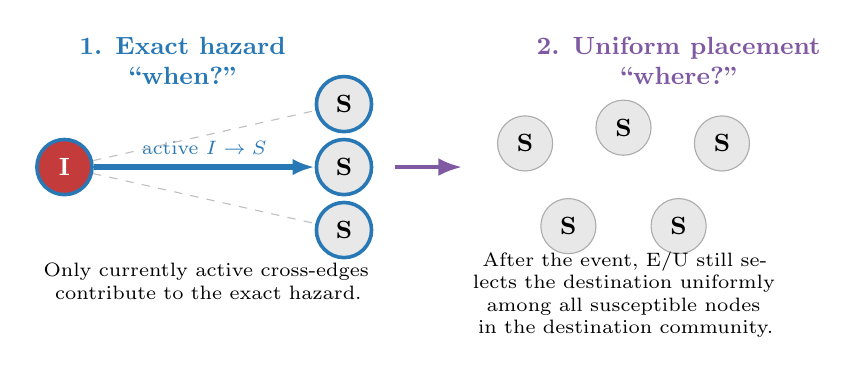
\begin{tikzpicture}[every node/.style={font=\small}]
\node[font=\bfseries\small,text=exact,align=center] at (1.75,2.25) {1. Exact hazard\\``when?''};
\node[ibnode,text=white,font=\bfseries\small] (a) at (0.25,0.9) {I};
\node[sbnode,font=\bfseries\small] (b1) at (3.8,0.9) {S}; \node[sbnode,font=\bfseries\small] (b2) at (3.8,1.7) {S}; \node[sbnode,font=\bfseries\small] (b3) at (3.8,0.1) {S};
\draw[exact,line width=2.3pt,-{Latex[length=2.8mm]}] (a)--node[above,font=\scriptsize] {active $I\to S$} (b1);
\draw[gray!50,dashed] (a)--(b2); \draw[gray!50,dashed] (a)--(b3);
\node[align=center,text width=43mm,font=\scriptsize] at (2.05,-0.55) {Only currently active cross-edges contribute to the exact hazard.};
\draw[-{Latex[length=3mm]},line width=1.4pt,purple] (4.45,0.9)--(5.3,0.9);
\node[font=\bfseries\small,text=purple,align=center] at (8.05,2.25) {2. Uniform placement\\``where?''};
\node[snode,font=\bfseries\small] (u1) at (6.1,1.2) {S}; \node[snode,font=\bfseries\small] (u2) at (7.35,1.4) {S}; \node[snode,font=\bfseries\small] (u3) at (8.6,1.2) {S}; \node[snode,font=\bfseries\small] (u4) at (6.65,0.15) {S}; \node[snode,font=\bfseries\small] (u5) at (8.05,0.15) {S};
\node[align=center,text width=45mm,font=\scriptsize] at (7.35,-0.72) {After the event, E/U still selects the destination uniformly among all susceptible nodes in the destination community.};
\end{tikzpicture}
\caption{E/U fixes only the hazard: exact active edges determine the event intensity, but the post-event target is still uniform.}
\end{figure}

On the baseline, replacing aggregate hazard with exact active-edge hazard increased RMST by about 59.6 relative to A/U, moving the diagnostic simulator toward Full Micro. A significant gap remained, about $-161.2$ RMST relative to Full Micro (95\% CI $[-266.8,-48.8]$). The remaining error is explained by placement: E/U knows \emph{when} a cross-community event should occur but can still put the import into the wrong susceptible node.

\section*{6. E/E: correct both hazard and placement}
E/E means
\[
E=\text{Exact hazard},\qquad E=\text{Exact placement}.
\]
The hazard is the same exact active-edge sum as in E/U. The difference is that when a cross-edge $(u,v)$ is selected, the infection is placed at its actual endpoint $v$. Thus E/E restores both the event intensity and the allowed destination endpoint.

The transition E/U$\to$E/E isolates the uniform-placement error: scheduler and exact hazard remain unchanged, while only target selection changes.

On the baseline, E/E was almost indistinguishable from Full Micro. The RMST difference was only about $+7.5$ with a 95\% CI of approximately $[-93.6,+120.3]$. E/U$\to$E/E increased RMST by about 168.8, moving propagation later and much closer to Full Micro. This indicates that, once hazard is correct, placement is a major remaining source of structural error.

\section*{7. What is the actual difference between E/E and Full Micro?}
After checking the implementations, this can be stated more strongly: \textbf{in Experiment 01, E/E and Full Micro are configured to implement the same CTMC generator}. They differ in code organization and random-number routing, not in the infection rules.

Full Micro receives the entire \texttt{full\_graph} and passes it to one \texttt{MicroEngine}. Internal and cross-community edges are simply edges of the same graph. Each active $u(I)-v(S)$ edge creates a channel
\[
a_{uv}=\beta w_{uv},
\]
and each infected node has recovery rate $\gamma$. All infection and recovery channels compete in one Gillespie race.

E/E also uses one global state for all nodes. Importantly, it does \textbf{not} contain a separate ``micro A simulator'' and ``micro B simulator''. The code only indexes edges into two groups: internal edges and cross-community edges. An active internal edge has rate $\beta_{\mathrm{in}}w$ and an active cross-edge has rate $\beta_{\mathrm{out}}w$.

The Experiment 01 runner explicitly requires
\[
\beta_{\mathrm{in}}=\beta_{\mathrm{out}},
\]
because Full Micro uses one infection rate for all graph edges. Recovery rules are the same as well.

\begin{figure}[h!]
\centering
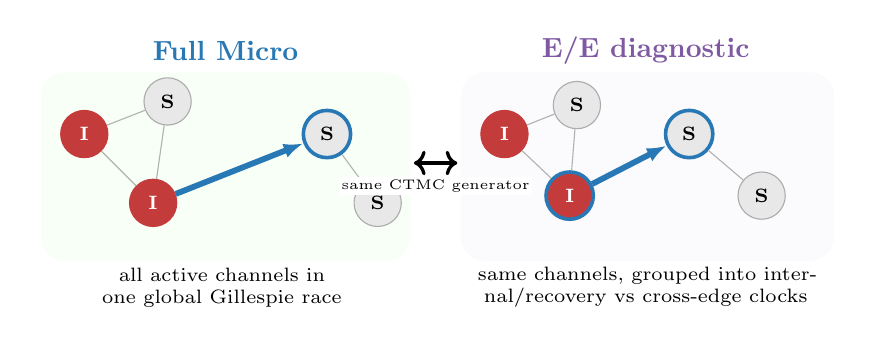
\begin{tikzpicture}[every node/.style={font=\small},scale=.92]
\node[font=\bfseries,text=exact] at (2.25,2.55) {Full Micro};
\fill[green!3,rounded corners=3mm] (-0.3,-0.35) rectangle (4.8,2.25);
\node[inode,text=white,font=\bfseries\scriptsize,minimum size=6mm] (f1) at (0.3,1.4) {I}; \node[snode,font=\bfseries\scriptsize,minimum size=6mm] (f2) at (1.45,1.85) {S}; \node[inode,text=white,font=\bfseries\scriptsize,minimum size=6mm] (f3) at (1.25,0.45) {I}; \node[sbnode,font=\bfseries\scriptsize,minimum size=6mm] (f4) at (3.65,1.4) {S}; \node[snode,font=\bfseries\scriptsize,minimum size=6mm] (f5) at (4.35,0.45) {S};
\draw[gray!60] (f1)--(f2)--(f3)--(f1); \draw[gray!60] (f4)--(f5); \draw[exact,line width=2.1pt,-{Latex[length=2.5mm]}] (f3)--(f4);
\node[font=\scriptsize,align=center,text width=47mm] at (2.2,-0.72) {all active channels in one global Gillespie race};
\node[font=\bfseries,text=purple] at (8.05,2.55) {E/E diagnostic};
\fill[purple!3,rounded corners=3mm] (5.5,-0.35) rectangle (10.65,2.25);
\node[inode,text=white,font=\bfseries\scriptsize,minimum size=6mm] (e1) at (6.1,1.4) {I}; \node[snode,font=\bfseries\scriptsize,minimum size=6mm] (e2) at (7.1,1.8) {S}; \node[ibnode,text=white,font=\bfseries\scriptsize,minimum size=6mm] (e3) at (7.0,0.55) {I}; \node[sbnode,font=\bfseries\scriptsize,minimum size=6mm] (e4) at (8.65,1.4) {S}; \node[snode,font=\bfseries\scriptsize,minimum size=6mm] (e5) at (9.65,0.55) {S};
\draw[gray!60] (e1)--(e2)--(e3)--(e1); \draw[gray!60] (e4)--(e5); \draw[exact,line width=2.1pt,-{Latex[length=2.5mm]}] (e3)--(e4);
\node[font=\scriptsize,align=center,text width=49mm] at (8.05,-0.72) {same channels, grouped into internal/recovery vs cross-edge clocks};
\draw[<->,line width=1.2pt] (4.85,1.0)--(5.45,1.0); \node[font=\tiny,fill=white,inner sep=1pt] at (5.15,.68) {same CTMC generator};
\end{tikzpicture}
\caption{E/E and Full Micro organize the channels differently in code, but in Experiment 01 they implement the same CTMC generator.}
\end{figure}

Let
\[
\Lambda_\mu=\Lambda_{\mathrm{internal}}+\Lambda_{\mathrm{recovery}},\qquad \Lambda_M=\Lambda_{\mathrm{cross}}.
\]
Full Micro samples one waiting time
\[
\Delta t\sim\mathrm{Exp}(\Lambda_\mu+\Lambda_M).
\]
E/E samples two independent times
\[
T_\mu\sim\mathrm{Exp}(\Lambda_\mu),\qquad T_M\sim\mathrm{Exp}(\Lambda_M)
\]
and takes the smaller. By the competing-exponentials identity,
\[
\min(T_\mu,T_M)\sim\mathrm{Exp}(\Lambda_\mu+\Lambda_M),
\]
and the probability that a group wins is proportional to its total rate. Thus the two scheduling procedures are mathematically equivalent.

For cross-community events, E/E also preserves the exact probability of selecting each active cross-edge. It first selects a community pair proportionally to the sum of rates of its active cross-edges, then selects the target proportionally to the total active-edge weight entering that target, and finally selects the source proportionally to the relevant edge weight. The resulting probability of choosing a concrete $(u,v)$ edge is the same as in Full Micro.

\begin{tcolorbox}[colback=soft,colframe=exact,title=No ``if the rules match'' qualifier is needed for Experiment 01]
The implementation itself enforces the equivalence conditions: same full graph and initial node, $\beta_{\mathrm{in}}=\beta_{\mathrm{out}}$, same $\gamma$, same SIR event rules, exact active cross-edge hazard, and exact edge-conditioned placement. Therefore E/E and Full Micro should have the same statistical distribution even though individual trajectories differ because RNG streams are organized differently.
\end{tcolorbox}

The oracle gate agrees with this: in 100 paired replications, Full Micro RMST was 2936.7 and E/E RMST was 2944.3; the difference was $+7.5$ with 95\% CI $[-93.6,+120.3]$, which includes zero.

\section*{8. One matched comparison of all simulator variants}
For v4, all available variants are combined into one matched comparison on the same 100 paired networks: $L=10$, $n=100$, $d\approx6$, $k=5$, $\beta_{\mathrm{in}}=\beta_{\mathrm{out}}=0.003$, SI dynamics, and $T_{\mathrm{end}}=4000$. The archived production and structural per-replication files use the same replication IDs; Full Micro values match exactly and EventDriven A/U matches A/U. Therefore the rows below refer to the same network realizations rather than different experimental samples.

All six variants reached the terminal community in all 100/100 runs before $T_{\mathrm{end}}=4000$, so there is no censoring in this distribution-first comparison.

\subsection*{8.1. Compare distributions, not only one average}
For simulator $m$, consider the complete terminal-arrival distribution
\[
F_m(t)=P(T_{\mathrm{last}}\le t).
\]
Median and IQR are retained as descriptive summaries, but the primary pairwise quantities are distances between distributions:
\begin{itemize}[nosep]
\item \textbf{Wasserstein-1 distance $W_1$}: the average amount of time-axis displacement needed to transform one empirical arrival-time distribution into another. It has the same time units as $T_{\mathrm{last}}$. Zero means identical empirical distributions.
\item \textbf{Kolmogorov--Smirnov distance $D_{KS}$}: the maximum vertical gap between two empirical CDFs. It ranges from 0 to 1; zero means identical ECDFs.
\end{itemize}
Distances are reported both relative to Full Micro and relative to \textbf{Production + independent RNG}, because corrected Production is now the main MicroMacro reference. P-values are deliberately not the central result here; for the paired-network design, distributional effect sizes are more informative.

\begin{landscape}
\begin{figure}[p]
\centering
\includegraphics[width=.96\linewidth]{v4_en_assets/distribution_table.png}
\caption{Distribution-first comparison of all six implementations on the same 100 paired networks. Mini-density plots use a common time axis from 0 to 4000 and a common vertical scale; the dotted line marks the median. Distances from Full Micro to corrected MicroMacro are shown as symmetric reference values, not as an ``error'' of Full Micro.}
\end{figure}
\end{landscape}

\subsection*{8.2. How to read the v4 comparison}
\textbf{Current shared-RNG Production} is an obvious outlier: $W_1=1259.2$ from Full Micro and $1051.9$ from corrected Production. It should no longer be used as the scientific MicroMacro baseline; it remains useful as evidence of the implementation bug.

\textbf{Production + independent RNG} brings the production implementation into the same time regime as diagnostic A/U and E/U. The distance from corrected Production to A/U is only $W_1=61.9$, $D_{KS}=0.12$; to E/U it is $W_1=50.4$, $D_{KS}=0.09$. This does not mean corrected Production \emph{is} E/U: it still uses aggregate hazard, uniform placement, and the production $\tau$-scheduler. It only means their marginal arrival-time distributions are close in this baseline.

\textbf{E/E is the closest to Full Micro}: $W_1=40.4$ and $D_{KS}=0.07$. This is a stronger statement than ``the averages are close'': the empirical terminal-arrival distributions themselves nearly coincide.

A/U and E/U lie between corrected Production and Full Micro. A/U$\to$E/U reduces $W_1$ to Full Micro from 220.8 to 163.6; E/U$\to$E/E reduces it further to 40.4. Thus the ablation ladder can be evaluated as progressive convergence of whole distributions, not merely a shift in a mean.

\subsection*{8.3. Structural ablation ladder}
Two distinct mechanisms can make production MicroMacro differ from Full Micro:
\begin{center}
\begin{tabular}{>{\raggedright\arraybackslash}p{30mm} >{\raggedright\arraybackslash}p{110mm}}
\textbf{Structural:} & exact boundary edges $\to$ aggregate community hazard.\\[2pt]
\textbf{Scheduler:} & global event competition $\to$ $\tau$-synchronized hazard integration.
\end{tabular}
\end{center}
A/U removes the production scheduler while retaining aggregate/uniform semantics. A/U$\to$E/U restores exact hazard. E/U$\to$E/E restores exact placement.

\begin{figure}[h!]
\centering
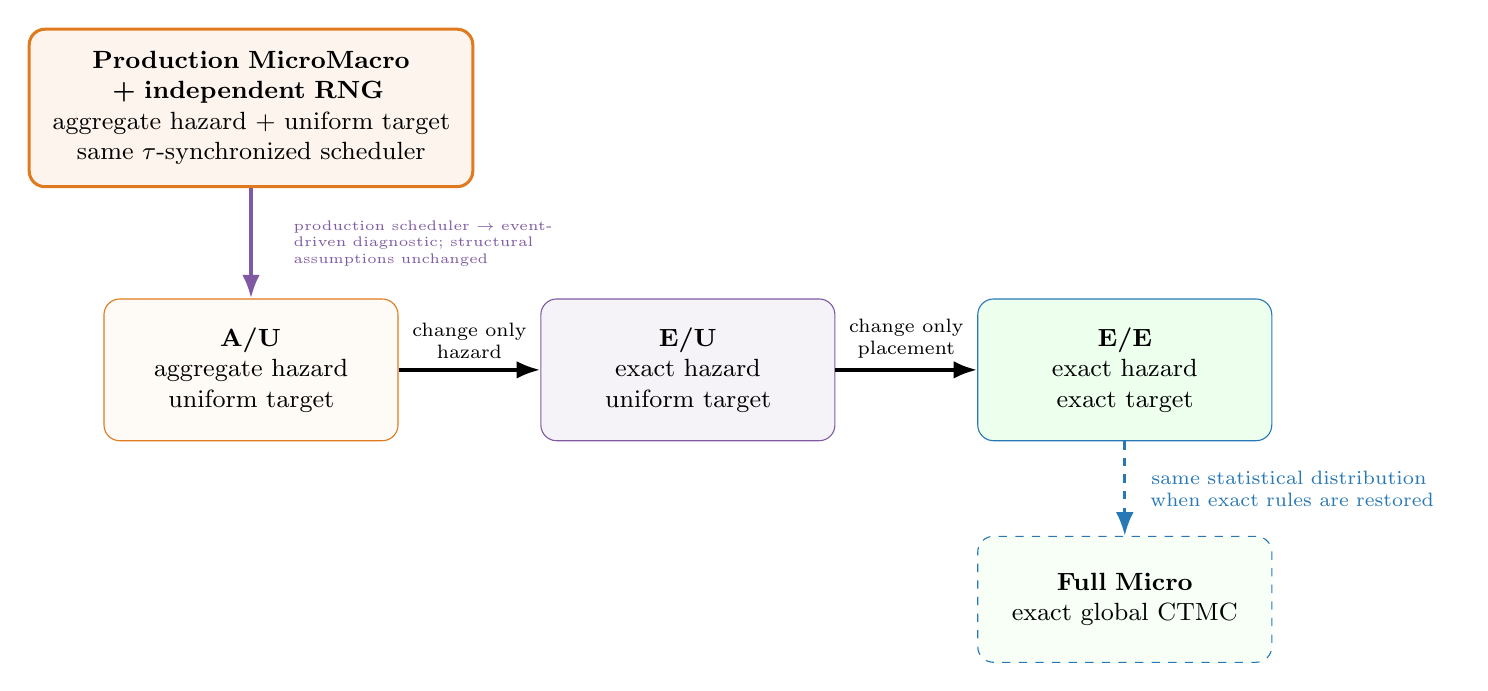
\begin{tikzpicture}[node distance=9mm and 7mm,every node/.style={font=\small}]
\node[rounded corners=2mm,draw=macro,line width=1.1pt,fill=macro!8,text width=54mm,minimum height=20mm,align=center] (prod) {\textbf{Production MicroMacro + independent RNG}\\aggregate hazard + uniform target\\same $\tau$-synchronized scheduler};
\node[rounded corners=2mm,draw=macro,fill=macro!4,text width=35mm,minimum height=18mm,align=center,below=14mm of prod] (au) {\textbf{A/U}\\aggregate hazard\\uniform target};
\draw[-{Latex[length=3mm]},line width=1.4pt,purple] (prod)--node[right=4mm,font=\tiny,align=left,text width=35mm,fill=white] {production scheduler $\to$ event-driven diagnostic; structural assumptions unchanged} (au);
\node[rounded corners=2mm,draw=purple,fill=purple!7,text width=35mm,minimum height=18mm,align=center,right=18mm of au] (eu) {\textbf{E/U}\\exact hazard\\uniform target};
\node[rounded corners=2mm,draw=exact,fill=green!7,text width=35mm,minimum height=18mm,align=center,right=18mm of eu] (ee) {\textbf{E/E}\\exact hazard\\exact target};
\draw[-{Latex[length=3mm]},line width=1.4pt] (au)--node[above,font=\scriptsize,align=center] {change only\\hazard} (eu);
\draw[-{Latex[length=3mm]},line width=1.4pt] (eu)--node[above,font=\scriptsize,align=center] {change only\\placement} (ee);
\node[rounded corners=2mm,draw=exact,dashed,fill=green!3,text width=35mm,minimum height=16mm,align=center,below=12mm of ee] (full) {\textbf{Full Micro}\\exact global CTMC};
\draw[-{Latex[length=3mm]},dashed,line width=1.1pt,exact] (ee)--node[right=2mm,font=\scriptsize,align=left,text width=38mm] {same statistical distribution when exact rules are restored} (full);
\end{tikzpicture}
\caption{What each step isolates in v4. The production baseline already uses independent RNG streams.}
\end{figure}

\section*{9. What should count as the main result for the paper?}
If the goal is to make claims about the user-facing MicroMacro method, the primary experiments should use the production \texttt{MicroMacroSimulator} with \textbf{independent RNG streams} and then modify only the minimum component needed for the particular ablation. The shared-RNG variant is no longer a valid scientific baseline.

\begin{center}
\begin{tabularx}{\textwidth}{>{\bfseries}p{35mm} X}
\toprule
Experiment & Cleanest implementation strategy\\
\midrule
A/U baseline & production MicroMacro + independent RNG streams; change nothing else\\
E/U & same corrected Production, replacing only the macro hazard provider with exact active-edge hazard\\
E/E & same corrected Production with exact hazard, replacing only the target selector with the exact edge endpoint\\
Gateway near/random/far & do not modify corrected Production; change topology only\\
$d\times k$ grid & do not modify corrected Production; change network parameters only\\
\bottomrule
\end{tabularx}
\end{center}

The separate \texttt{HazardPlacementSimulator} remains very useful as a secondary mechanistic diagnostic because it removes production scheduler artifacts and cleanly decomposes structural error. But it should be presented as mechanism validation rather than the only evidence for what a user of corrected production MicroMacro will observe.

\section*{10. Shortest possible summary}
\begin{itemize}[leftmargin=*,itemsep=4pt]
\item \textbf{Full Micro}: sees every node and every active edge. Exact hazard, exact target.
\item \textbf{Production MicroMacro (primary v4 reference)}: original architecture with independent RNG streams for micro communities; between communities it uses aggregate $I,S,W$, aggregate hazard, uniform target, and the production $\tau$-scheduler.
\item \textbf{Shared-RNG Production}: same intended architecture but with a confirmed RNG-coupling bug; keep only as a historical/bug reference.
\item \textbf{Structural A/U}: same aggregate/uniform structural assumptions in a separate event-driven diagnostic simulator; it removes the production $\tau$-scheduler while retaining structural A/U approximation.
\item \textbf{E/U}: same diagnostic scheduler and uniform placement, but aggregate hazard is replaced by exact cross-edge hazard; A/U$\to$E/U isolates hazard-information loss.
\item \textbf{E/E}: same diagnostic scheduler and exact hazard, but uniform placement is replaced by the exact endpoint; E/U$\to$E/E isolates placement error. In Experiment 01 it implements the same CTMC generator as Full Micro.
\end{itemize}

\section*{Source note}
The description of production MicroMacro, its two layers, macro-rate, and cumulative-hazard synchronization is based on \emph{Towards complexity reduction of large-scale epidemic simulation in two-scale networks} (MoMLeT-2025). The Full Micro description is based on \emph{Simulating epidemic peak dynamics on complex networks using efficient Gillespie algorithms}. The distinction between Structural A/U--E/U--E/E is based on the audited experiment source code. Earlier RMST values come from Experiment 01 (hazard/placement factorial ablation, 100 paired replications) and Experiment 07 (production implementation decomposition). The v4 distribution-first comparison reuses the archived per-replication results; no new simulation run was needed.

\end{document}
